%!TEX root = da-screen.tex

Covering maps can be used to argue that a problem cannot be solved at all. Now we will study a technique that can be used to argue that a problem cannot be solved \emph{fast}.

Some problems can be solved very quickly with a distributed algorithm. For example, algorithm $\algo{VC3}$ from Section~\ref{ssec:vc3} runs in time $O(\Delta)$, where $\Delta$ is the maximum degree of the graph. If we focus on a family of bounded-degree graphs, i.e., $\Delta = O(1)$, this is a constant-time algorithm\mydash the running time of the algorithm is independent of the size of the graph.

\section{An Introductory Example}\label{sec:local-neighbourhood-example}

However, some problems cannot be solved quickly with any distributed algorithm. As an introductory example, let $\calF$ consist of all path graphs, and let $\Pi$ be the problem of finding a $2$-edge colouring.
\begin{center}
    \includegraphics[page=\PTwoEdgeCol]{figs.pdf}
\end{center}

With a little thought, we can design a distributed algorithm $A$ that solves $\Pi$ on $\calF$. Informally, algorithm $A$ proceeds as follows. First, we find the midpoint of the graph. This is possible if nodes of degree $1$ generate a token that is forwarded by nodes of degree $2$. Eventually, the two tokens meet at the midpoint of the graph. There are two cases:
\begin{enumerate}
    \item The midpoint is a node $v$, i.e., we have an even path. Then we can use the port numbers of $v$ to break symmetry: the edge connected to port $i$ is labelled with colour $i$. Then we can assign alternating colours to all other edges, starting from $v$.
    \item The midpoint is an edge $\{u,v\}$, i.e., we have an odd path. Then we can assign colour $1$ to $\{u,v\}$ and alternating colours to all other edges, starting from both $u$ and $v$.
\end{enumerate}

The algorithm certainly finds a correct solution\mydash in any path graph, the edges will be properly coloured with colours $1$ and~$2$. However, the running time of the algorithm is $\Theta(n)$, where $n$ is the number of nodes.

We will now argue that no algorithm can find a $2$-edge colouring in time $o(n)$. To this end, assume that $G$ is a path of length $2r+3$, and let $N$ be a simple port-numbered network that has $G$ as the underlying graph; choose the port numbers as shown in Figure~\ref{fig:path-same-neigh}.

\begin{figure}
    \centering
    \includegraphics[page=\PPathSameNeigh]{figs.pdf}
    \caption{Nodes $u$ and $v$ have isomorphic radius-$r$ neighbourhoods in a path of length $2r+3$; in this illustration, $r = 2$.}\label{fig:path-same-neigh}
\end{figure}

Now let $u$ and $v$ be the two nodes that are incident to the midpoint of the path. Let us label the nodes in the radius-$r$ neighbourhoods of $u$ and $v$ as we have shown in Figure~\ref{fig:path-same-neigh}:
\begin{align*}
    \ball_G(u,r) &= \Set{u_{-r}, u_{-r+1}, \dotsc, u_r}, \\
    \ball_G(v,r) &= \Set{v_{-r}, v_{-r+1}, \dotsc, v_r}.
\end{align*}
In particular, $v = v_0$ and $u = u_0$.

Now assume that we have a distributed algorithm $A$, and we apply it to $N$. Initially, we have
\[
    x_0(u_i) = x_0(v_i) \quad \text{for all}\quad{-r} \le i \le r.
\]
It follows that the messages sent by $u_i$ and $v_i$ on round $1$ are identical for all $-r \le i \le r$. Therefore the messages received by $u_i$ and $v_i$ on round $1$ are identical for all $-r+1 \le i \le r-1$ (note that $u_r$ and $v_r$ may receive different messages). It follows that after round $1$ we have
\[
    x_1(u_i) = x_1(v_i) \quad \text{for all}\quad{-r+1} \le i \le r-1.
\]
By induction, after round $t \le r$ we have
\[
    x_t(u_i) = x_t(v_i) \quad \text{for all}\quad{-r+t} \le i \le r-t.
\]
In particular,
\[
    x_r(u) = x_r(u_0) = x_r(v_0) = x_r(v).
\]
Hence if $A$ stops in time $r$, both $u$ and $v$ produce the same output. However, this contradicts with the definition of problem $\Pi$. Therefore the running time of $A$ has to be larger than $r$ in a graph with $2r+4$ nodes.

In what follows, we will formalise and generalise the ideas that we used in this example.

\section{Definitions}

Let $N = (V,P,p)$ and $N' = (V'\!,P'\!,p')$ be simple port-numbered networks, with the underlying graphs $G = (V,E)$ and $G' = (V'\!,E')$. Fix the local inputs $f\colon V \to Y$ and $f'\colon V' \to Y$, a pair of nodes $v \in V$ and $v' \in V'$, and a radius $r \in \NN$. Define the radius-$r$ neighbourhoods
\[
    U = \ball_G(v,r), \quad U' = \ball_{G'}(v'\!,r).
\]
We say that $(N,f,v)$ and $(N'\!,f'\!,v')$ have \emph{isomorphic radius-$r$ neighbourhoods} if there is a bijection $\psi \colon U \to U'$ with $\psi(v) = v'$ such that
\begin{enumerate}\raggedright
    \item $\psi$ preserves degrees: $\deg_{N}(v) = \deg_{N'}(\psi(v))$ for~all~$v \in U$.
    \item $\psi$ preserves connections and port numbers: $p(u,i) = (v,j)$ if and only if $p'(\psi(u),i) = (\psi(v),j)$ for~all~$u, v \in U$.
    \item $\psi$ preserves local inputs: $f(v) = f'(\psi(v))$ for~all~$v \in U$.
\end{enumerate}
The function $\psi$ is called an \emph{$r$-neighbourhood isomorphism from $(N,f,v)$ to $(N'\!,f'\!,v')$}. See Figure~\ref{fig:same-neigh} for an example.

\begin{figure}
    \centering
    \includegraphics[page=\PSameNeigh]{figs.pdf}
    \caption{Nodes $u$ and $v$ have isomorphic radius-$2$ neighbourhoods, provided that we choose the port numbers appropriately. Therefore in any algorithm $A$ the state of $u$ equals the state of $v$ at time $t = 0,1,2$. However, at time $t = 3, 4, \dotsc$ this does not necessarily hold.}\label{fig:same-neigh}
\end{figure}

\section{Local Neighbourhoods and Executions}

\begin{theorem}\label{thm:local-neighbourhood}
    Assume that
    \begin{enumerate}[itemsep=0ex]\raggedright
        \item $A$ is a distributed algorithm with $X = \Input_A$,
        \item $N = (V,P,p)$ and $N' = (V'\!,P'\!,p')$ are simple port-numbered networks,
        \item $f\colon V \to X$ and $f'\colon V' \to X$ are arbitrary functions,
        \item $v \in V$ and $v' \in V'$,
        \item $(N,f,v)$ and $(N'\!,f'\!,v')$ have isomorphic radius-$r$ neighbourhoods.
    \end{enumerate}
    Let
    \begin{enumerate}[resume*]
        \item $x_0, x_1, \dotsc$ be the execution of $A$ on $(N,f)$, and
        \item $x'_0, x'_1, \dotsc$ be the execution of $A$ on $(N'\!,f')$.
    \end{enumerate}
    Then for each $t = 0, 1, \dotsc, r$ we have $x_t(v) = x'_t(v')$.
\end{theorem}

\begin{proof}
    Let $G$ and $G'$ be the underlying graphs of $N$ and $N'$, respectively. We will prove the following stronger claim by induction: for each $t = 0, 1, \dotsc, r$, we have $x_t(u) = x'_t(\psi(u))$ for all $u \in \ball_G(v,r-t)$.
    
    To prove the base case $t = 0$, let $u \in \ball_G(v,r)$, $d = \deg_N(u)$, and $u' = \psi(u)$; we have
    \[
        x'_0(u') = \Init_{A,d}(f'(u')) = \Init_{A,d}(f(u)) = x_0(u).
    \]
    
    For the inductive step, assume that $t \ge 1$ and \[u \in \ball_G(v,r-t).\] Let $u' = \psi(u)$. By inductive assumption, we have
    \[
        x'_{t-1}(u') = x_{t-1}(u).
    \]
    Now consider a port $(u,i) \in P$. Let $(s,j) = p(u,i)$. We have $\{s,u\} \in E$, and therefore
    \[
        \dist_G(s,v) \le \dist_G(s,u) + \dist_G(u,v) \le 1 + r-t.
    \]
    Define $s' = \psi(s)$. By inductive assumption we have
    \[
        x'_{t-1}(s') = x_{t-1}(s).
    \]
    The neighbourhood isomorphism $\psi$ preserves the port numbers: $(s',j) = p'(u',i)$. Hence all of the following are equal:
    \begin{enumerate}[noitemsep]
        \item the message sent by $s$ to port $j$ on round $t$,
        \item the message sent by $s'$ to port $j$ on round $t$,
        \item the message received by $u$ from port $i$ on round $t$,
        \item the message received by $u'$ from port $i$ on round $t$.
    \end{enumerate}
    As the same holds for any port of $u$, we conclude that
    \[
        x'_t(u') = x_t(u). \qedhere
    \]
\end{proof}

We will often consider the case that $N = N'$ but $v \ne v'$ when we apply Theorem~\ref{thm:local-neighbourhood}; we have already seen an example of this in Section~\ref{sec:local-neighbourhood-example}.


\section{Exercises}

\begin{ex}[path graphs]
    In this exercise, the graph family $\calF$ consists of \emph{path graphs}.
    \begin{subex}
        \item Show that it is possible to find a maximum matching in time $3n+O(1)$.
        \item Show that it is not possible to find a maximum matching in time $n/3+O(1)$.
        \item Show that it is not possible to find a $2$-colouring.
        \item Show that it is not possible to find a weak $2$-colouring.
        \item Is it possible to find a minimum vertex cover? If yes, how fast?
        \item Is it possible to find a minimum dominating set? If yes, how fast?
        \item Is it possible to find a minimum edge dominating set? If yes, how fast?
        \item How fast is it possible to find a \Apx{2} of a minimum vertex cover?
        \item How fast is it possible to find a \Apx{2} of a minimum dominating set?
    \end{subex}
\end{ex}

\begin{ex}[path graphs with auxiliary information]
    In this exercise, the graph family $\calF$ consists of \emph{path graphs}.
    \begin{subex}
        \item Assume that we are given a $4$-colouring. Show that it is possible to find a $3$-colouring in time $1$.
        \item Assume that we are given a $4$-colouring. Show that it is not possible to find a $3$-colouring in time $0$.
        \item Assume that we are given a $4$-colouring. Show that it is possible to find a $2$-colouring in time $3n+O(1)$.
        \item Assume that we are given a $4$-colouring. Show that it is not possible to find a $2$-colouring in time $n/3+O(1)$.
        \item Assume that we are given a $4$-colouring. How fast is it possible to find a weak $2$-colouring?
        \item Assume that we are given an orientation. Show that it is possible to find a $2$-colouring in time $3n+O(1)$.
        \item Assume that we are given an orientation. Show that it is not possible to find a $2$-colouring in time $n/3+O(1)$.
    \end{subex}
\end{ex}

\begin{ex}[combining techniques]\label{ex:neigh-ex}
    Consider the graphs $G_1$ and $G_2$ illustrated in Figure~\ref{fig:neigh-ex}. Show that there are simple port-numbered networks $N_1$ and $N_2$ such that $N_i$ has $G_i$ as the underlying graph, and in any distributed algorithm with running time $2$ the output of $v_1$ in $N_1$ equals the output of $v_2$ in~$N_2$.

    \hint{We need to combine the results of Theorems \ref{thm:cover} and \ref{thm:local-neighbourhood}. For $i = 1,2$, construct a network $N'_i$ and a covering map $\phi_i$ from $N'_i$ to $N_i$. Let $v'_i \in \phi^{-1}_i(v_i)$. Show that $v'_1$ and $v'_2$ have isomorphic radius-$2$ neighbourhoods; hence $v'_1$ and $v'_2$ produce the same output. Then use the covering maps to argue that $v_1$ and $v_2$ also produce the same outputs. In the construction of $N'_1$, you will need to eliminate the $3$-cycle; otherwise $v'_1$ and $v'_2$ cannot have isomorphic neighbourhoods.}

    \begin{figure}
        \centering
        \includegraphics[page=\PNeighEx]{figs.pdf}
        \caption{Graphs for Exercise~\ref{ex:neigh-ex}.}\label{fig:neigh-ex}
    \end{figure}
\end{ex}

